% !TeX program = xelatex
\documentclass[a4paper,10pt]{article}

% ============================================================================
% កញ្ចប់ស្នូល និងការកំណត់ទំព័រ (តាមគំរូ ls_plan.tex ១០០%)
% ============================================================================
\usepackage[a4paper, left=0.95cm, right=0.95cm, top=0.85cm, bottom=0.92cm, footskip=0.52cm]{geometry}
\usepackage{amsmath}
\usepackage{unicode-math}
\usepackage{fontspec}
\usepackage{longtable, array, colortbl}
\usepackage[table]{xcolor}
\usepackage{enumitem}
\usepackage{pifont}
\usepackage{fancyhdr}
\usepackage{tikz}
\usetikzlibrary{calc, arrows.meta, angles, quotes, patterns, decorations.markings, babel}

\makeatletter
\let\@expl@@@mark@update@singlecol@structures@@\relax
\makeatother

% ============================================================================
% ការកំណត់ពុម្ពអក្សរ (Cross-Platform Font Resolver: Windows Local + Linux Cloud)
% ============================================================================
\providecommand{\NGSFindFonts}{%
  \IfFileExists{C:/Windows/Fonts/cambria.ttc}{%
    \def\NGSSysPath{C:/Windows/Fonts/}%
    \def\NGSUserPath{C:/Users/KIT/AppData/Local/Microsoft/Windows/Fonts/}%
  }{%
    \IfFileExists{./fonts/KhmerOSsiemreap.ttf}{\def\NGSSysPath{./fonts/}\def\NGSUserPath{./fonts/}}{%
    \IfFileExists{../fonts/KhmerOSsiemreap.ttf}{\def\NGSSysPath{../fonts/}\def\NGSUserPath{../fonts/}}{%
    \IfFileExists{../../fonts/KhmerOSsiemreap.ttf}{\def\NGSSysPath{../../fonts/}\def\NGSUserPath{../../fonts/}}{%
    \IfFileExists{../../../fonts/KhmerOSsiemreap.ttf}{\def\NGSSysPath{../../../fonts/}\def\NGSUserPath{../../../fonts/}}{%
    \IfFileExists{../../../../fonts/KhmerOSsiemreap.ttf}{\def\NGSSysPath{../../../../fonts/}\def\NGSUserPath{../../../../fonts/}}{%
    \IfFileExists{../../../../../fonts/KhmerOSsiemreap.ttf}{\def\NGSSysPath{../../../../../fonts/}\def\NGSUserPath{../../../../../fonts/}}{%
    \IfFileExists{../../../../../../fonts/KhmerOSsiemreap.ttf}{\def\NGSSysPath{../../../../../../fonts/}\def\NGSUserPath{../../../../../../fonts/}}{%
      \def\NGSSysPath{../../../../../../../fonts/}\def\NGSUserPath{../../../../../../../fonts/}%
    }}}}}}}%
  }%
}
\NGSFindFonts

\setmathfont[Path={\NGSSysPath}, FontIndex=1, Scale=1.02]{cambria.ttc}
\defaultfontfeatures{Ligatures=TeX}

\setmainfont[
  Path={\NGSUserPath},
  Extension=.ttf,
  Script=Khmer,
  BoldFont={KhmerOSsiemreap},
  BoldFeatures={FakeBold=1.8},
  ItalicFont={KhmerOSsiemreap},
  ItalicFeatures={FakeSlant=0.25},
  BoldItalicFont={KhmerOSsiemreap},
  BoldItalicFeatures={FakeBold=1.8, FakeSlant=0.25}
]{KhmerOSsiemreap}

\newfontfamily\muol[
  Path={\NGSUserPath},
  Extension=.ttf,
  Script=Khmer
]{KhmerOSmuollight}

\newfontfamily\Tacteing[
  Path={\NGSUserPath},
  Extension=.TTF
]{TACTENG}

\newfontfamily\TimesEn[
  Path={\NGSSysPath},
  Extension=.ttf,
  Scale=1.00,
  BoldFont={timesbd},
  ItalicFont={timesi},
  BoldItalicFont={timesbi}
]{times}

\newfontfamily\NagaBold[
  Path={\NGSUserPath},
  Extension=.ttf
]{AKbalthom Naga Bold}

\newfontfamily\CalibriFont[
  Path={\NGSSysPath},
  Extension=.ttf
]{calibri}

\newfontfamily\CourierBullet[
  Path={\NGSSysPath},
  Extension=.ttf
]{cour}
\newcommand{\wcirc}{{\CourierBullet\fontsize{9.5pt}{11pt}\selectfont o}}

\XeTeXlinebreaklocale "km"
\XeTeXlinebreakskip = 0pt plus 1pt minus 0.1pt

% ============================================================================
% ពណ៌ ប្លង់ទំព័រ និងម៉ាក្រូជំនួយ
% ============================================================================
\definecolor{stepgray}{HTML}{D9D9D9}
\definecolor{headgray}{HTML}{F2F2F2}
\definecolor{boxgray}{HTML}{E6E6E6}
\definecolor{darkred}{HTML}{C00000}
\definecolor{red5e}{HTML}{FF0000}

\pagestyle{fancy}
\fancyhf{}
\renewcommand{\headrulewidth}{0pt}
\fancyfoot[R]{\CalibriFont\fontsize{11pt}{13pt}\selectfont\thepage}

\setlength{\parindent}{0pt}
\setlength{\parskip}{0pt}
\setlength{\tabcolsep}{3.8pt}
\setlength{\LTpre}{2pt}
\setlength{\LTpost}{2pt}

\newcolumntype{L}[1]{>{\raggedright\arraybackslash}p{#1}}
\newcolumntype{C}[1]{>{\centering\arraybackslash}p{#1}}

\newcommand{\en}[1]{{\TimesEn #1}}
\newcommand{\enbf}[1]{{\TimesEn\textbf{#1}}}
\newcommand{\unit}[1]{\,\text{\en{#1}}}
\newcommand{\fiveE}[1]{{\NagaBold\fontsize{9.5pt}{13pt}\selectfont\textcolor{red5e}{#1}}}
\newcommand{\timenote}[1]{\textcolor{darkred}{\textit{#1}}}
\newcommand{\khmflourish}{{\Tacteing\fontsize{17pt}{17pt}\selectfont 3}}
\newcommand{\graybox}[1]{\colorbox{boxgray}{\strut\hspace{2pt}#1\hspace{2pt}}}
\newcommand{\ditem}{\tikz[baseline=-0.5ex]\fill (0,0.42ex) -- (0.42ex,0) -- (0,-0.42ex) -- (-0.42ex,0) -- cycle;\hspace{0.3em}}
\newcommand{\cnum}[1]{{\fontsize{10.5pt}{12pt}\selectfont\ding{\numexpr181+#1\relax}}\hspace{0.2em}}
\newcommand{\cfig}[1]{\par\vspace{4pt}{\centering #1\par}\vspace{4pt}}
\newcommand{\stepheader}[1]{\multicolumn{3}{|c|}{\cellcolor{stepgray}\muol #1} \\* \noalign{\hrule height 0.4pt}}
\newcommand{\tri}[1]{\ensuremath{\triangle #1}}
\newcommand{\ang}[1]{\ensuremath{\angle #1}}
\newcommand{\chkbox}{\tikz[baseline=-0.15ex]\draw[black, line width=0.8pt] (0,0) rectangle (0.23cm,0.23cm);}

\newcommand{\rightbox}[4][0.18]{%
  \draw[black, line width=0.75pt]
    ($(#3)!#1!(#2)$) -- ($($(#3)!#1!(#2)$)+($(#3)!#1!(#4)$)-(#3)$) -- ($(#3)!#1!(#4)$);
}

\tikzset{
  tk1/.style={postaction={decorate},decoration={markings,mark=at position 0.50 with {\draw[black, line width=0.85pt](0,-0.09)--(0,0.09);}}},
  tk2/.style={postaction={decorate},decoration={markings,
    mark=at position 0.45 with {\draw[black, line width=0.85pt](0,-0.09)--(0,0.09);},
    mark=at position 0.55 with {\draw[black, line width=0.85pt](0,-0.09)--(0,0.09);}}}
}

% ============================================================================
% រូបធរណីមាត្រ ស-ខ្មៅ (B&W Print-Safe TikZ Figures for Hour 17.2: Pyramids)
% ============================================================================

% ១. កំណែកិច្ចការផ្ទះទី៣ (ទំ.២២៧) និងរំលឹកទ្រឹស្ដីបទពីតាករ (ទំ.២១៨)
\newcommand{\figPrereqPyr}{%
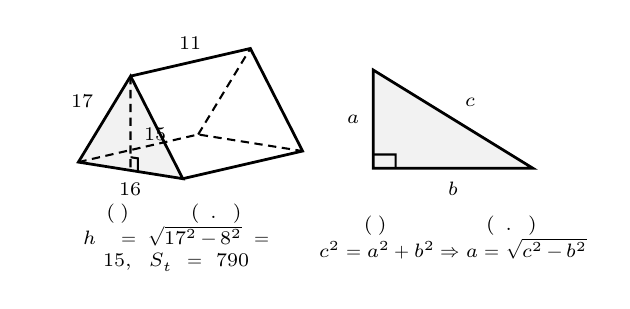
\begin{tikzpicture}[scale=0.78, every node/.style={font=\scriptsize, text=black}]
  % (ក) លំហាត់ទី៣ ទំ.២២៧៖ ព្រីសត្រង់ត្រីមុខបាតត្រីកោណសមបាត 17, 17, 16 និងទ្រនុងខាង 11
  \begin{scope}[shift={(0,0)}]
    \coordinate (A) at (-1.50,-0.65);
    \coordinate (B) at (0.20,-0.92);
    \coordinate (C) at (-0.65,0.75);
    \coordinate (M) at ($0.5*(A)+0.5*(B)$);
    \coordinate (S) at (1.95,0.45);
    \fill[gray!10] (A) -- (B) -- (C) -- cycle;
    \draw[black, line width=1.0pt] (A) -- (B) -- (C) -- cycle;
    \draw[black, line width=1.0pt] (B) -- ($(B)+(S)$) -- ($(C)+(S)$) -- (C);
    \draw[black, line width=0.75pt, densely dashed] (A) -- ($(A)+(S)$) -- ($(B)+(S)$) ($(A)+(S)$) -- ($(C)+(S)$);
    \draw[black, line width=0.8pt, densely dashed] (C) -- (M);
    \rightbox[0.14]{C}{M}{B}
    \node[above left=0.5pt] at ($0.5*(A)+0.5*(C)$) {$17$};
    \node[right=1.5pt] at ($0.38*(C)+0.62*(M)$) {$15$};
    \node[below=1pt] at (M) {$16$};
    \node[above=1pt] at ($0.5*(C)+0.5*(C)+0.5*(S)$) {$11$};
    \node[align=center, text width=3.55cm] at (0.10,-1.88) {(ក) លំហាត់ទី៣ (ទំ.២២៧)៖\\$h_{\text{បាត}}=\sqrt{17^2-8^2}=15,\; S_t=790$};
  \end{scope}

  % (ខ) ទ្រឹស្ដីបទពីតាករ និងព្រីសទល់នឹងពីរ៉ាមីត
  \begin{scope}[shift={(4.65,0)}]
    \coordinate (P) at (-1.35,-0.75);
    \coordinate (Q) at (1.25,-0.75);
    \coordinate (R) at (-1.35,0.85);
    \fill[gray!10] (P) -- (Q) -- (R) -- cycle;
    \draw[black, line width=1.0pt] (P) -- (Q) -- (R) -- cycle;
    \rightbox[0.14]{R}{P}{Q}
    \node[left=1.5pt] at ($0.5*(P)+0.5*(R)$) {$a$};
    \node[below=1.5pt] at ($0.5*(P)+0.5*(Q)$) {$b$};
    \node[above right=1pt] at ($0.5*(Q)+0.5*(R)$) {$c$};
    \node[align=center, text width=3.55cm] at (-0.05,-1.88) {(ខ) ទ្រឹស្ដីបទពីតាករ (ទំ.២១៨)៖\\$c^2 = a^2 + b^2 \Rightarrow a = \sqrt{c^2-b^2}$};
  \end{scope}
\end{tikzpicture}}

% ២. E1 Engage: ដំបូលខ្ចូសរាងពីរ៉ាមីតចតុមុខនិយ័ត (លំហាត់គំរូទី 1 ទំ.២១៩៖ ទ្រនុងខាង 10 ទល់នឹងអាប៉ូតែម SH)
\newcommand{\figEngagePyr}{%
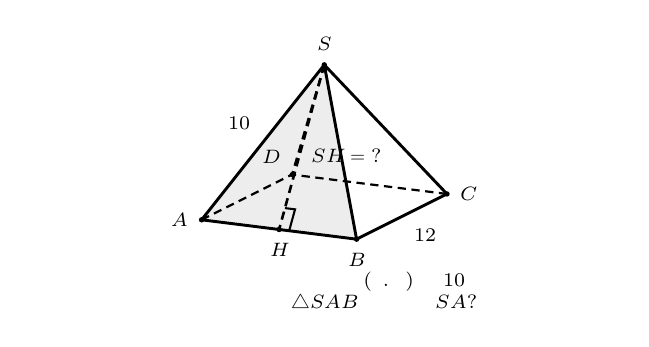
\begin{tikzpicture}[scale=0.82, every node/.style={font=\scriptsize, text=black}]
  \coordinate (A) at (-1.85,-0.75);
  \coordinate (B) at (0.55,-1.05);
  \coordinate (C) at (1.95,-0.35);
  \coordinate (D) at (-0.45,-0.05);
  \coordinate (O) at ($0.5*(A)+0.5*(C)$);
  \coordinate (S) at (0.05,1.65);
  \coordinate (H) at ($0.5*(A)+0.5*(B)$);

  \fill[gray!14] (S) -- (A) -- (B) -- cycle;
  \draw[black, line width=1.05pt] (A) -- (B) -- (C);
  \draw[black, line width=0.8pt, densely dashed] (A) -- (D) -- (C);
  \draw[black, line width=1.05pt] (S) -- (A) (S) -- (B) (S) -- (C);
  \draw[black, line width=0.8pt, densely dashed] (S) -- (D);
  \draw[black, line width=0.95pt, densely dashed] (S) -- (H);
  \rightbox[0.13]{S}{H}{B}

  \fill[black] (S) circle (1.2pt) node[above=1.5pt] {$S$};
  \fill[black] (A) circle (1.2pt) node[left=1.5pt] {$A$};
  \fill[black] (B) circle (1.2pt) node[below=1.5pt] {$B$};
  \fill[black] (C) circle (1.2pt) node[right=1.5pt] {$C$};
  \fill[black] (D) circle (1.1pt) node[above left=0.5pt] {$D$};
  \fill[black] (H) circle (1.2pt) node[below=1.5pt] {$H$};

  \node[above left=1pt] at ($0.5*(S)+0.5*(A)$) {$10$};
  \node[below right=1pt] at ($0.5*(B)+0.5*(C)$) {$12$};
  \node[right=1pt] at ($0.45*(S)+0.55*(H)$) {$SH=?$};

  \node[align=center, text width=7.3cm] at (0.05,-1.85) {ដំបូលខ្ចូសរាងពីរ៉ាមីតចតុមុខនិយ័ត (ទំ.២១៩)៖ តើ $10$ ជាកម្ពស់ត្រីកោណមុខខាង $\tri{SAB}$ ឬជាទ្រនុងខាង $SA$?};
\end{tikzpicture}}

% ៣. E2/E3 ការប្រៀបធៀប កម្ពស់ h, អាប៉ូតែម d និងជនេត្រ/ទ្រនុងខាង (ទំ.២១៨) + គំនូសលាតផ្កាយ 2D (គំរូទី 1)
\newcommand{\figPyrBridgeNet}{%
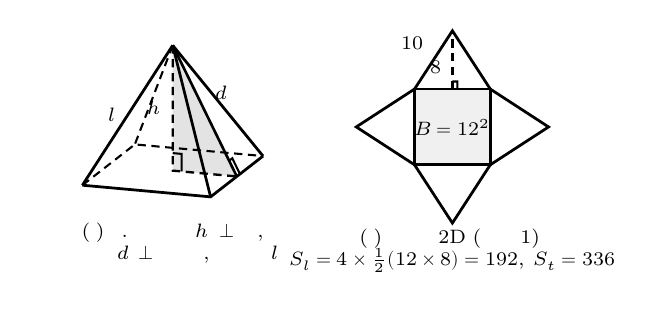
\begin{tikzpicture}[scale=0.74, every node/.style={font=\scriptsize, text=black}]
  % (ក) ត្រីកោណកែងក្នុងពីរ៉ាមីត៖ កម្ពស់ SO, អាប៉ូតែម SH, ទ្រនុងខាង SB
  \begin{scope}[shift={(-2.55,0)}]
    \coordinate (A) at (-1.55,-0.95);
    \coordinate (B) at (0.65,-1.15);
    \coordinate (C) at (1.55,-0.45);
    \coordinate (D) at (-0.65,-0.25);
    \coordinate (O) at (0.0,-0.70);
    \coordinate (S) at (0.0,1.45);
    \coordinate (H) at (1.10,-0.80);

    \fill[gray!22] (S) -- (O) -- (H) -- cycle;
    \draw[black, line width=1.0pt] (A) -- (B) -- (C);
    \draw[black, line width=0.75pt, densely dashed] (A) -- (D) -- (C);
    \draw[black, line width=1.0pt] (S) -- (A) (S) -- (B) (S) -- (C);
    \draw[black, line width=0.75pt, densely dashed] (S) -- (D);
    \draw[black, line width=0.95pt] (S) -- (H);
    \draw[black, line width=0.85pt, densely dashed] (S) -- (O) -- (H);
    \rightbox[0.14]{S}{O}{H}
    \rightbox[0.12]{S}{H}{C}

    \node[left=1pt] at ($0.5*(S)+0.5*(O)$) {$h$};
    \node[above right=0.5pt] at ($0.5*(S)+0.5*(H)$) {$d$};
    \node[left=1pt] at ($0.5*(S)+0.5*(A)$) {$l$};
    \node[align=center, text width=3.45cm] at (0.0,-1.95) {(ក) ទំ.២១៨៖ កម្ពស់ $h\perp$ បាត,\\អាប៉ូតែម $d\perp$ ជ្រុងបាត, ទ្រនុងខាង $l$};
  \end{scope}

  % (ខ) គំនូសលាតផ្កាយ 2D នៃលំហាត់គំរូទី 1 (បាតការេ 12x12 + ត្រីកោណសមបាត 4 ដែល d=8)
  \begin{scope}[shift={(2.25,0.05)}]
    \draw[black, line width=1.0pt, fill=gray!12] (-0.65,-0.65) rectangle (0.65,0.65);
    % ត្រីកោណមុខខាងទាំង 4
    \draw[black, line width=1.0pt] (-0.65,0.65) -- (0,1.65) -- (0.65,0.65);
    \draw[black, line width=1.0pt] (-0.65,-0.65) -- (0,-1.65) -- (0.65,-0.65);
    \draw[black, line width=1.0pt] (-0.65,-0.65) -- (-1.65,0) -- (-0.65,0.65);
    \draw[black, line width=1.0pt] (0.65,-0.65) -- (1.65,0) -- (0.65,0.65);
    \draw[black, line width=0.8pt, densely dashed] (0,0.65) -- (0,1.65);
    \coordinate (NTop) at (0,1.65);
    \coordinate (NMid) at (0,0.65);
    \coordinate (NRt) at (0.65,0.65);
    \rightbox[0.13]{NTop}{NMid}{NRt}
    \node at (0,0) {$B=12^2$};
    \node[left=0.5pt] at (0,1.02) {$8$};
    \node[above left=0pt] at (-0.32,1.15) {$10$};
    \node[align=center, text width=4.15cm] at (0.0,-2.12) {(ខ) លាតផ្កាយ \en{2D} (គំរូទី \en{1})៖\\$S_l=4\times\frac{1}{2}(12\times 8)=192,\; S_t=336$};
  \end{scope}
\end{tikzpicture}}

% ៤. E4 លំហាត់គំរូទី 2 (ទំ.២១៩-២២០), ប្រតិបត្តិ (ទំ.២២០) និងលំហាត់ទី៤ (ទំ.២២៧)
\newcommand{\figElaboratePyr}{%
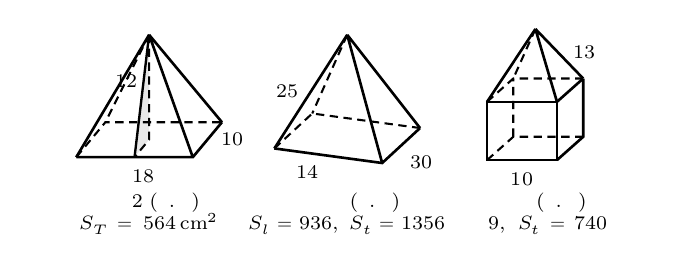
\begin{tikzpicture}[scale=0.74, every node/.style={font=\scriptsize, text=black}]
  % (១) លំហាត់គំរូទី 2៖ បាត 10x18, កម្ពស់ AF=12 => AG=15, AH=13
  \begin{scope}[shift={(-3.10,0)}]
    \coordinate (C) at (-1.15,-0.85);
    \coordinate (D) at (0.85,-0.85);
    \coordinate (E) at (1.35,-0.25);
    \coordinate (B) at (-0.65,-0.25);
    \coordinate (F) at (0.10,-0.55);
    \coordinate (A) at (0.10,1.25);
    \coordinate (H) at (-0.15,-0.85);
    \fill[gray!18] (A) -- (F) -- (H) -- cycle;
    \draw[black, line width=0.95pt] (C) -- (D) -- (E) (A) -- (C) (A) -- (D) (A) -- (E);
    \draw[black, line width=0.75pt, densely dashed] (C) -- (B) -- (E) (A) -- (B) (A) -- (F) -- (H);
    \draw[black, line width=0.85pt] (A) -- (H);
    \node[below=1pt] at (0.0,-0.85) {$18$};
    \node[right=1pt] at (1.12,-0.55) {$10$};
    \node[left=0.5pt] at (0.10,0.45) {$12$};
    \node[align=center, text width=2.85cm] at (0.10,-1.82) {គំរូទី \en{2} (ទំ.២២០)៖\\$S_T=564\unit{cm}^2$};
  \end{scope}

  % (២) ប្រតិបត្តិ ទំ.២២០៖ បាត 14x30, ទ្រនុងខាង 25 => d1=24, d2=20
  \begin{scope}[shift={(0.35,0)}]
    \coordinate (P1) at (-1.20,-0.70);
    \coordinate (P2) at (0.65,-0.95);
    \coordinate (P3) at (1.30,-0.35);
    \coordinate (P4) at (-0.55,-0.10);
    \coordinate (V) at (0.05,1.25);
    \draw[black, line width=0.95pt] (P1) -- (P2) -- (P3) (V) -- (P1) (V) -- (P2) (V) -- (P3);
    \draw[black, line width=0.75pt, densely dashed] (P1) -- (P4) -- (P3) (V) -- (P4);
    \node[left=1pt] at ($0.5*(V)+0.5*(P1)$) {$25$};
    \node[below left=0pt] at ($0.5*(P1)+0.5*(P2)$) {$14$};
    \node[below right=0pt] at ($0.5*(P2)+0.5*(P3)$) {$30$};
    \node[align=center, text width=2.85cm] at (0.05,-1.82) {ប្រតិបត្តិ (ទំ.២២០)៖\\$S_l=936,\; S_t=1356$};
  \end{scope}

  % (៣) លំហាត់ទី៤ ទំ.២២៧៖ សូលីតផ្សំ គូបជ្រុង 10 + ពីរ៉ាមីតនិយ័តទ្រនុងខាង 13
  \begin{scope}[shift={(3.55,0)}]
    \draw[black, line width=0.95pt] (-0.75,-0.90) rectangle (0.45,0.10);
    \draw[black, line width=0.95pt] (0.45,-0.90) -- (0.90,-0.50) -- (0.90,0.50);
    \draw[black, line width=0.95pt] (0.45,0.10) -- (0.90,0.50);
    \draw[black, line width=0.75pt, densely dashed] (-0.75,0.10) -- (-0.30,0.50) -- (0.90,0.50);
    \draw[black, line width=0.75pt, densely dashed] (-0.75,-0.90) -- (-0.30,-0.50) -- (0.90,-0.50) (-0.30,-0.50) -- (-0.30,0.50);
    \coordinate (TopP) at (0.08,1.35);
    \draw[black, line width=0.95pt] (TopP) -- (-0.75,0.10) (TopP) -- (0.45,0.10) (TopP) -- (0.90,0.50);
    \draw[black, line width=0.75pt, densely dashed] (TopP) -- (-0.30,0.50);
    \node[below=1pt] at (-0.15,-0.90) {$10$};
    \node[right=1pt] at (0.52,0.95) {$13$};
    \node[align=center, text width=2.55cm] at (0.10,-1.82) {លំហាត់ទី៤ (ទំ.២២៧)៖\\មុខ $9,\; S_t=740$};
  \end{scope}
\end{tikzpicture}}

% ============================================================================
% ចាប់ផ្ដើមឯកសារ (Document Body)
% ============================================================================
\begin{document}
\fontsize{10pt}{15.2pt}\selectfont

% -------------------- ក្បាលកិច្ចតែងការ (Header) --------------------
\begin{center}
  {\muol\fontsize{11pt}{16pt}\selectfont ព្រះរាជាណាចក្រកម្ពុជា}\\[2pt]
  {\muol\fontsize{10pt}{15pt}\selectfont ជាតិ សាសនា ព្រះមហាក្សត្រ}\\[1pt]
  \khmflourish
\end{center}

\vspace{-26pt}
{\muol\fontsize{9.5pt}{12.8pt}\selectfont
មន្ទីរអប់រំ យុវជន និងកីឡា ខេត្តកំពង់ធំ\\
ការិយាល័យអប់រំ យុវជន និងកីឡា ស្រុកកំពង់ស្វាយ\\
អនុវិទ្យាល័យព្រះក្រសាំង}

\vspace{1pt}
\begin{center}
  {\muol\fontsize{10pt}{14.5pt}\selectfont កិច្ចតែងការបង្រៀន}
\end{center}
\vspace{0pt}

% -------------------- ព័ត៌មានទូទៅ (Metadata) --------------------
{\renewcommand{\arraystretch}{0.98}
\hspace*{4.05cm}%
\begin{tabular}{@{}l l l@{}}
  - \hspace{0.35cm} មុខវិជ្ជា & : & គណិតវិទ្យា ថ្នាក់ទី៨ \\
  - \hspace{0.35cm} ចំណងជើងមេរៀន & : & មេរៀនទី១៧ រូបធរណីមាត្រដែលមានវិមាត្របី \\
  - \hspace{0.35cm} ចំណងជើងរង & : & ១៧.១ ផ្ទៃក្រឡាខាងនិងផ្ទៃក្រឡាទាំងអស់នៃពីរ៉ាមីត (ទំព័រ ២១៨--២២០) \\
  - \hspace{0.35cm} រយៈពេល & : & ១ ម៉ោងសិក្សា (៥០ នាទី) \\
  - \hspace{0.35cm} បង្រៀនដោយ & : & ហុក ប៊ុនថែន \\
  - \hspace{0.35cm} កាលបរិច្ឆេទ & : & ថ្ងៃ\makebox[18mm]{\dotfill}\ ទី\makebox[8mm]{\dotfill}\ ខែ\makebox[18mm]{\dotfill}\ ឆ្នាំ២០២៦ \\
\end{tabular}

\vspace{2pt}

% -------------------- I. វត្ថុបំណង --------------------
\textbf{I.} {\muol វត្ថុបំណង}\\[1pt]
\hspace*{0.55cm}%
\begin{tabular}{@{}l l L{14.2cm}@{}}
  \wcirc \hspace{0.25cm} វិជ្ជាសម្បទា & : & សិស្សប្រាប់បានត្រឹមត្រូវពីធាតុនៃពីរ៉ាមីត និងពីរ៉ាមីតនិយ័ត (កំពូល បាតតែមួយ មុខខាងជាត្រីកោណ កម្ពស់ អាប៉ូតែម និងជនេត្រ/ទ្រនុងខាង) ព្រមទាំងរូបមន្តផ្ទៃក្រឡាខាង ($S_l$) និងផ្ទៃក្រឡាទាំងអស់ ($S_t = S_l + B$) នៃពីរ៉ាមីត ។ \\
  \wcirc \hspace{0.25cm} បំណិនសម្បទា & : & សិស្សប្រើទ្រឹស្ដីបទពីតាករគណនាអាប៉ូតែមនៃមុខខាងត្រីកោណ (ទាំងពីរ៉ាមីតនិយ័ត និងពីរ៉ាមីតបាតចតុកោណកែង) និងគណនាផ្ទៃក្រឡាខាង ផ្ទៃក្រឡាទាំងអស់ ព្រមទាំងសូលីតផ្សំលើសន្លឹកកិច្ចការបានត្រឹមត្រូវ ។ \\
  \wcirc \hspace{0.25cm} ចរិយាសម្បទា & : & សិស្សមានភាពម៉ត់ចត់ក្នុងការបែងចែករវាងកម្ពស់ពីរ៉ាមីត ទ្រនុងខាង និងអាប៉ូតែមមុខខាង ដោយមិនយកទ្រនុងខាងមកជំនួសកម្ពស់ត្រីកោណមុខខាងដោយប្រហែស ។ \\
\end{tabular}

\vspace{2pt}

% -------------------- II. សម្ភារៈឧបទេស --------------------
\textbf{II.} {\muol សម្ភារៈឧបទេស}\\[1pt]
\hspace*{0.55cm}$\bullet$ \hspace{0.35cm} សៀវភៅសិក្សាគោលគណិតវិទ្យាថ្នាក់ទី៨ (ទំ.២១៨--២២០ និង ២២៧--២២៨) សន្លឹកកិច្ចការសិស្ស ស-ខ្មៅ (\en{Worksheet\_PYR\_SA} ចំនួន ២ ទំព័រ គ្មាន \en{LCD}) ក្ដារខៀន ដីស បន្ទាត់ក្រិត និងអេគែរ ។

\vspace{2pt}

% -------------------- III. វិធីសាស្រ្តបង្រៀន --------------------
\textbf{III.} {\muol វិធីសាស្រ្តបង្រៀន}\\[1pt]
\hspace*{0.45cm}%
\begin{tabular}{@{}l l L{14.85cm}@{}}
  $\bullet$ \hspace{0.25cm} គោលវិធី & : & សិស្សមជ្ឈមណ្ឌល (សិក្សាតាមរយៈការបំពេញលើសន្លឹកកិច្ចការជាគោល គ្មាន \en{LCD} និងគ្មានការកាត់បិទក្រដាស) \\
  $\bullet$ \hspace{0.25cm} យុទ្ធវិធីបង្រៀន & : & ស្ថាបនានិយម គម្រូ \en{5Es} រួមបញ្ចូលការលាតប្លង់ផ្កាយ \en{2D} (\en{Star-Net Decomposition}), ស្ពានពីតាកររកអាប៉ូតែម (\en{Pythagorean Slant-Height Bridge}) និងការវិភាគមុខបាំងកំបាំងនៃសូលីតផ្សំ ។ \\
\end{tabular}
}

\vspace{2pt}

% -------------------- IV. ដំណើរការបង្រៀន --------------------
\textbf{IV.} {\muol ដំណើរការបង្រៀន}

\vspace{1pt}

\renewcommand{\arraystretch}{1.15}
\begin{longtable}{|L{5.50cm}|L{7.90cm}|L{4.80cm}|}
\hline
\rowcolor{headgray}
\multicolumn{1}{|c|}{\muol សកម្មភាពគ្រូ} &
\multicolumn{1}{c|}{\muol ខ្លឹមសារមេរៀន} &
\multicolumn{1}{c|}{\muol សកម្មភាពសិស្ស} \\
\hline
\endfirsthead

\hline
\rowcolor{headgray}
\multicolumn{1}{|c|}{\muol សកម្មភាពគ្រូ} &
\multicolumn{1}{c|}{\muol ខ្លឹមសារមេរៀន} &
\multicolumn{1}{c|}{\muol សកម្មភាពសិស្ស} \\
\hline
\endhead

\hline
\endfoot

\hline
\endlastfoot

% ==================== ជំហានទី១ (2 min) ====================
\stepheader{ជំហានទី១ (រដ្ឋបាលថ្នាក់)}
$\bullet$ ពិនិត្យវត្តមាន សណ្ដាប់ធ្នាប់ អនាម័យ និងចែកសន្លឹកកិច្ចការ \en{Worksheet\_PYR\_SA} ដល់សិស្សគ្រប់គូ \timenote{(2 min)}
&
$\bullet$ រដ្ឋបាលថ្នាក់ និងការត្រៀមសៀវភៅគោល បន្ទាត់ក្រិត អេគែរ និងសន្លឹកកិច្ចការសិស្ស
&
$\circ$ ប្រធានថ្នាក់រាយការណ៍វត្តមាន\par\vspace{2pt}
$\circ$ ទទួលសន្លឹកកិច្ចការ និងត្រៀមឧបករណ៍ \\[3pt]
\hline

% ==================== ជំហានទី២ (9 min: ≤3 + 3 + E1 3) ====================
\stepheader{ជំហានទី២ (កិច្ចការផ្ទះ + រំលឹកមេរៀនចាស់ + ទំនាក់ទំនងមេរៀនថ្មី)}
\timenote{(កំណែកិច្ចការផ្ទះ $\le 3\text{ min}$)}\par\vspace{1pt}
$\bullet$ ពិនិត្យចម្លើយលំហាត់ទី១ខ (ទំ.២២៦) និងលំហាត់ទី៣ (ទំ.២២៧) លើក្ដារខៀនយ៉ាងរហ័ស
&
\textbf{កំណែកិច្ចការផ្ទះ (ទំ.២២៦--២២៧ លំហាត់ទី១ខ និងទី៣)៖}\par\vspace{1pt}
$1.$ \textbf{ទី១ខ៖} $S_l = 2(12+8)\times 13 = 520\unit{mm}^2 \Rightarrow S_t = 520+2(96) = \mathbf{712\unit{mm}^2}$ ។\par\vspace{1pt}
$2.$ \textbf{ទី៣៖} $S_l = (17+17+16)\times 11 = 550$;\; $h_{\text{បាត}}=\sqrt{17^2-8^2}=15 \Rightarrow B=\frac{16\times 15}{2}=120 \Rightarrow S_t = 550+240 = \graybox{$790$}$ ។
&
$\circ$ ផ្ទៀងផ្ទាត់និងកែកំណែលំហាត់ទី១ខ និងទី៣ ក្នុងសៀវភៅ \\[3pt]

\timenote{(រំលឹកមេរៀនចាស់ 3 min)}\par\vspace{1pt}
$\bullet$ សួរ៖ «តើព្រីសមានបាតប៉ុន្មាន? ចុះក្នុងត្រីកោណកែងដែលមានអ៊ីប៉ូតេនុស $c$ និងជ្រុងកែងមួយ $b$ តើជ្រុងកែង $a$ រកតាមរូបមន្តអ្វី?»
&
\textbf{រំលឹកព្រីស និងទ្រឹស្ដីបទពីតាករ (ទំ.២១៦ និង ២១៨)៖}\par\vspace{1pt}
\ditem ព្រីសមានបាត \textbf{២} ស្របគ្នាប៉ុនគ្នា ($S_t = S_l + 2B$) ។\par\vspace{1pt}
\ditem ទ្រឹស្ដីបទពីតាករ៖ $c^2 = a^2 + b^2 \Rightarrow a = \sqrt{c^2 - b^2}$ ។
&
$\circ$ ឆ្លើយរំលឹកចំនួនបាតព្រីស និងរូបមន្តពីតាករ \\[3pt]

& \cfig{\figPrereqPyr} & \\[3pt]

\fiveE{E1 - Engage} \timenote{(3 min)}\par\vspace{1.5pt}
$\bullet$ បង្ហាញបញ្ហាដំបូលខ្ចូសលើ \textbf{បេសកកម្មទី១ (\en{E1})} នៃសន្លឹកកិច្ចការ៖\par\vspace{1pt}
\hspace*{0.3em}-- «ដំបូលខ្ចូសរាងពីរ៉ាមីតចតុមុខនិយ័តមានជ្រុងបាតការេ $AB=12$ និងផ្លានជ្រុង (ទ្រនុងខាង) $SA=10$ ។ ជាង ក គណនាផ្ទៃមុខខាងមួយស្មើ $\frac{1}{2}\times 12\times 10=60$ ឯជាង ខ ថាខុស ព្រោះ $10$ មិនមែនជាកម្ពស់ត្រីកោណមុខខាង $SH$ ទេ! តើជាងណាត្រឹមត្រូវ?»
&
\textbf{១៧.១ ផ្ទៃក្រឡាខាង និងផ្ទៃក្រឡាទាំងអស់នៃពីរ៉ាមីត}\par\vspace{1.5pt}
\ditem \textbf{បញ្ហាបំផុសគំនិត (\en{E1})៖} ការបែងចែកឱ្យដាច់រវាង \textbf{ទ្រនុងខាង/ជនេត្រ} ($SA=10$) និង \textbf{អាប៉ូតែម} ($SH\perp AB$) ពេលគណនាផ្ទៃត្រីកោណមុខខាងនៃពីរ៉ាមីត ។
&
$\circ$ អានបេសកកម្មទី១ ពិនិត្យរូបដំបូលខ្ចូស និងគូសធីកទស្សន៍ទាយជាដៃគូ \\[3pt]

& \cfig{\figEngagePyr} & \\[3pt]
\hline

% ==================== ជំហានទី៣ (17 min: E2 11 + E3 6) ====================
\stepheader{ជំហានទី៣ (ខ្លឹមសារមេរៀនថ្មី)}
\fiveE{E2 - Explore} \timenote{(11 min: 5 min)}\par\vspace{1pt}
$\bullet$ ឱ្យសិស្សធ្វើជាដៃគូលើ \textbf{ផ្នែកទី១ (ក) បែងចែកធាតុទាំង ៣ នៃពីរ៉ាមីត និងគំនូសលាតផ្កាយ \en{2D}} (ទំ.២១៨)
&
\textbf{សកម្មភាពរុករកទី១ (ធាតុនៃពីរ៉ាមីត និងគំនូសលាតផ្កាយ \en{2D})៖}\par\vspace{1pt}
$1.$ ពីរ៉ាមីតមាន \textbf{បាតតែមួយគត់} ហើយទ្រនុងខាងប្រសព្វគ្នាត្រង់ \textbf{កំពូល} $S$ (មុខខាងសុទ្ធតែជាត្រីកោណ) ។
&
$\circ$ ពិនិត្យរូបពីរ៉ាមីត និងគំនូសលាតផ្កាយ \en{2D} លើសន្លឹកកិច្ចការ \\[3pt]

$\bullet$ ដើរសួរ៖ «តើកម្ពស់ពីរ៉ាមីត $SO$, អាប៉ូតែម $SH$ និងជនេត្រ/ទ្រនុងខាង $SA$ ខុសគ្នាដូចម្ដេច?»
&
$2.$ \textbf{កម្ពស់ $h=SO$} កែងនឹងបាតត្រង់ផ្ចិត $O$; \textbf{អាប៉ូតែម $d=SH$} ជាកម្ពស់ត្រីកោណមុខខាងកែងនឹងជ្រុងបាតត្រង់ចំណុចកណ្ដាល $H$; ឯ \textbf{ជនេត្រ/ទ្រនុងខាង $SA$} ភ្ជាប់កំពូលទៅកំពូលបាត!
&
$\circ$ កំណត់ឈ្មោះអង្កត់ $SO, SH, SA$ លើសន្លឹកកិច្ចការបានត្រឹមត្រូវ \\[3pt]

\timenote{(E2 ទី២៖ ស្ពានពីតាករលើលំហាត់គំរូទី \en{1} — 6 min)}\par\vspace{1.5pt}
$\bullet$ ដឹកនាំសិស្សបំពេញ \textbf{ផ្នែកទី១ (ខ) ស្ពានពីតាកររកអាប៉ូតែម $SH$} ក្នុងលំហាត់គំរូទី \en{1} (ទំ.២១៩៖ $AB=12, SA=10$)
&
\textbf{សកម្មភាពរុករកទី២ — លំហាត់គំរូទី \en{1} (ទំ.២១៩)៖}\par\vspace{1.5pt}
$\bullet$ $H$ កណ្ដាល $AB \Rightarrow AH = \frac{12}{2} = 6$ ។ តាមពីតាករក្នុង $\tri{SAH}$ កែងត្រង់ $H$៖\par\vspace{1pt}
\hspace*{0.2em}$AH^2 + SH^2 = SA^2 \Rightarrow SH^2 = 10^2 - 6^2 = 64 \Rightarrow \mathbf{SH = 8}$ (អាប៉ូតែម) ។
&
$\circ$ អនុវត្តទ្រឹស្ដីបទពីតាកររកឃើញអាប៉ូតែម $SH = 8 < 10$ \\[3pt]

$\bullet$ សួរបន្ត៖ «ពេលស្គាល់អាប៉ូតែម $SH=8$ តើផ្ទៃក្រឡាខាង $S_l$ និងផ្ទៃក្រឡាទាំងអស់ $S_t$ នៃពីរ៉ាមីតស្មើប៉ុន្មាន?»
&
$\bullet$ ក. ផ្ទៃក្រឡាខាង៖ $S_l = 4 \times \dfrac{1}{2}\times (8\times 12) = \mathbf{192}$ ឯកតាផ្ទៃ ។\par\vspace{1pt}
$\bullet$ ខ. ផ្ទៃក្រឡាទាំងអស់ (បាតតែ ១!)៖ $S_t = S_l + B = 192 + 12^2 = \graybox{$336\text{ ឯកតាផ្ទៃ}$}$ ។
&
$\circ$ គណនាបាន $S_l = 192$ និង $S_t = 336$ ឯកតាផ្ទៃ \\[3pt]

& \cfig{\figPyrBridgeNet} & \\[3pt]

\fiveE{E3 - Explain} \timenote{(6 min)}\par\vspace{1.5pt}
$\bullet$ ហៅតំណាងគូបង្ហាញ រួចគ្រូសង្ខេបនិយមន័យពីរ៉ាមីត និងពីរ៉ាមីតនិយ័ត (ទំ.២១៨) ឱ្យសិស្សបំពេញ \textbf{ផ្នែកទី២}
&
\textbf{និយមន័យ និងលក្ខណៈពីរ៉ាមីតនិយ័ត (ទំ.២១៨)៖}\par\vspace{1.5pt}
$\bullet$ \textbf{ពីរ៉ាមីតនិយ័ត៖} មានបាតជាពហុកោណនិយ័ត និងទ្រនុងខាងទាំងអស់ប៉ុនគ្នា $\Rightarrow$ មុខខាងទាំងអស់ជា \textbf{ត្រីកោណសមបាតប៉ុនគ្នា} (មានអាប៉ូតែម $d$ ស្មើគ្នា) ។\par\vspace{1pt}
$\bullet$ បើបាតជាចតុកោណកែងមិនស្មើជ្រុង ($l\neq w$) នោះវា \textbf{មិនមែន} ជាពីរ៉ាមីតនិយ័តទេ (មុខខាងមានអាប៉ូតែម ២ គូខុសគ្នា)!
&
$\circ$ តំណាងគូឡើងបកស្រាយ\par\vspace{2pt}
$\circ$ បំពេញនិយមន័យនិងចំណាំក្នុងផ្នែកទី២ \\[3pt]

$\bullet$ សង្ខេបរូបមន្តផ្ទៃក្រឡាពីរ៉ាមីត និងធនាគារហេតុផល \cnum{1}--\cnum{4}
&
\textbf{រូបមន្តផ្ទៃក្រឡានៃពីរ៉ាមីត៖}\par\vspace{1.5pt}
$\bullet$ ផ្ទៃក្រឡាខាង៖ $S_l = \text{ផលបូកផ្ទៃមុខខាងទាំងអស់}$ (បើពីរ៉ាមីតនិយ័ត៖ \graybox{$S_l = \dfrac{1}{2}P \times d$}) ។\par\vspace{1.5pt}
$\bullet$ ផ្ទៃក្រឡាទាំងអស់៖ \graybox{$S_t = S_l + B$} (បាតតែ \textbf{១} គត់ ខុសពីព្រីស $2B$!) ។\par\vspace{1.5pt}
$\bullet$ \textbf{ធនាគារហេតុផល៖} \cnum{1} ពីតាកររកអាប៉ូតែម $d$ \;\textbar\; \cnum{2} $S_l = \sum S_{\text{មុខខាង}}$ (ឬ $\frac{1}{2}Pd$) \;\textbar\; \cnum{3} $S_t = S_l + B$ \;\textbar\; \cnum{4} ដកមុខត្រួតគ្នាក្នុងសូលីតផ្សំ
&
$\circ$ បំពេញប្រអប់រូបមន្ត $S_l, S_t$ និងផ្ទៀងផ្ទាត់ធនាគារហេតុផល \cnum{1}--\cnum{4} \\[3pt]
\hline

% ==================== ជំហានទី៤ (20 min: E4 10 + E5 10) ====================
\stepheader{ជំហានទី៤ (ពង្រីកចំណេះដឹង និងវាយតម្លៃ)}
\fiveE{E4 - Elaborate} \timenote{(10 min: 5 min)}\par\vspace{1pt}
$\bullet$ ដឹកនាំសិស្សដោះស្រាយ \textbf{ផ្នែកទី៣ (ក) លំហាត់គំរូទី \en{2} (ទំ.២១៩--២២០)}៖ បាតចតុកោណកែង $10\unit{cm}\times 18\unit{cm}$ និងកម្ពស់ $AF=12\unit{cm}$
&
\textbf{៣.ក លំហាត់គំរូទី \en{2} (ទំ.២១៩--២២០ — បាតចតុកោណកែង)៖}\par\vspace{1.5pt}
$\bullet$ ក. មិនមែនពីរ៉ាមីតចតុមុខនិយ័តទេ ព្រោះបាត $BCDE$ ($10\times 18$) មិនមែនជាការេ ។\par\vspace{1pt}
$\bullet$ ខ. អាប៉ូតែមទាំងពីរ៖ ក្នុង $\tri{AFG}$: $AG=\sqrt{12^2+9^2}=\mathbf{15\unit{cm}}$; ក្នុង $\tri{AFH}$: $AH=\sqrt{12^2+5^2}=\mathbf{13\unit{cm}}$ ។\par\vspace{1pt}
\hspace*{0.2em}$\Rightarrow S_T = 2\cdot\frac{1}{2}(18\times 13) + 2\cdot\frac{1}{2}(10\times 15) + (10\times 18) = 234+150+180 = \graybox{$564\unit{cm}^2$}$ ។
&
$\circ$ គណនាអាប៉ូតែមទាំងពីរ ($15\unit{cm}, 13\unit{cm}$) និងផ្ទៃសរុប $564\unit{cm}^2$ \\[3pt]

\timenote{(E4 ទី២៖ ប្រតិបត្តិ ទំ.២២០ — 5 min)}\par\vspace{1.5pt}
$\bullet$ ឱ្យសិស្សធ្វើជាដៃគូលើ \textbf{ផ្នែកទី៣ (ខ) ប្រតិបត្តិ (ទំ.២២០)}៖ បាតចតុកោណកែង $14\unit{cm}\times 30\unit{cm}$ និងទ្រនុងខាង $25\unit{cm}$
&
\textbf{៣.ខ ប្រតិបត្តិ (ទំ.២២០)៖}\par\vspace{1.5pt}
$\bullet$ ក. មិនមែនពីរ៉ាមីតនិយ័តទេ (បាត $14\unit{cm}\neq 30\unit{cm}$) ។\par\vspace{1pt}
$\bullet$ ខ. អាប៉ូតែមលើជ្រុង $14$: $d_1 = \sqrt{25^2-7^2} = 24\unit{cm}$; លើជ្រុង $30$: $d_2 = \sqrt{25^2-15^2} = 20\unit{cm}$ ។\par\vspace{1pt}
\hspace*{0.2em}\mbox{\ditem $S_l =$} $(14\times 24) + (30\times 20) = 336 + 600 = \mathbf{936\unit{cm}^2}$ ។\par\vspace{1pt}
$\bullet$ គ. $S_t = 936 + (14\times 30) = 936 + 420 = \graybox{$1356\unit{cm}^2$}$ ។
&
$\circ$ រក $d_1=24\unit{cm},\; d_2=20\unit{cm}$ រួចគណនា $S_l=936\unit{cm}^2$ និង $S_t=1356\unit{cm}^2$ \\[3pt]

& \cfig{\figElaboratePyr} & \\[3pt]

\fiveE{E5 - Evaluate} \timenote{(10 min: 6 min)}\par\vspace{1pt}
$\bullet$ ឱ្យសិស្សធ្វើ \textbf{ផ្នែកទី៤ (ក) លំហាត់សូលីតផ្សំទី៤ ក, ខ (ទំ.២២៧)} ដោយឯករាជ្យលើសន្លឹកកិច្ចការ
&
\textbf{រង្វាយតម្លៃទី១ — លំហាត់ទី៤ ក, ខ (ទំ.២២៧៖ គូបជ្រុង $10$ + ពីរ៉ាមីតទ្រនុងខាង $13$)៖}\par\vspace{1.5pt}
$1.$ \textbf{ក.} $ABCD$ \textbf{មិនមែន} ជាមុខនៃសូលីតផ្សំទេ ព្រោះវាស្ថិតនៅខាងក្នុងត្រួតគ្នារវាងគូបនិងពីរ៉ាមីត! \textbf{ខ.} ចំនួនមុខសរុប $= 5\text{ (គូប)} + 4\text{ (ពីរ៉ាមីត)} = \graybox{$9\text{ មុខ}$}$ ។
&
$\circ$ វិភាគរូបសូលីតផ្សំ ឆ្លើយ ក (មិនមែន) និង ខ ($9$ មុខ) \\[3pt]

$\bullet$ ដើរពិនិត្យការរកអាប៉ូតែមពីរ៉ាមីតលើកំពូលគូប ជាស្ពានសម្រាប់កិច្ចការផ្ទះសំណួរ គ
&
$2.$ អាប៉ូតែមពីរ៉ាមីតលើគូប៖ $d = \sqrt{13^2 - 5^2} = \sqrt{144} = \mathbf{12} \Rightarrow S_{l,\text{ពីរ៉ាមីត}} = 4\times\frac{1}{2}(10\times 12) = \graybox{$240\text{ ឯកតាផ្ទៃ}$}$ ។
&
$\circ$ គណនាអាប៉ូតែម $d=12$ និងផ្ទៃដំបូលពីរ៉ាមីត $240$ \\[3pt]

\timenote{(E5 បិទបេសកកម្ម \en{E1} និង \en{Exit Check} — 4 min)}\par\vspace{1.5pt}
$\bullet$ សួរបិទបេសកកម្មដំបូលខ្ចូស \en{E1} និងឱ្យសិស្សគូសវង់ \textbf{\en{Exit Check} (ផ្នែកទី៤ ខ)} ដើម្បីវាយតម្លៃរហ័ស
&
\textbf{រង្វាយតម្លៃទី២ — បិទ \en{E1} និង \en{Exit Check}៖}\par\vspace{1.5pt}
$\bullet$ \textbf{ចម្លើយ \en{E1}៖} \textbf{ជាង ខ ត្រឹមត្រូវ} — $10$ ជាទ្រនុងខាង $SA$; អាប៉ូតែមពិតគឺ $SH=\sqrt{10^2-6^2}=8 \Rightarrow$ ផ្ទៃមុខខាងមួយ $= \frac{1}{2}(12\times 8)=48$ (មិនមែន $60$ ទេ)! \par\vspace{1pt}
$\bullet$ \textbf{\en{Exit Check}៖} សំណួរទី១ $\to$ \textbf{ខ} ($S_t = S_l + B$); សំណួរទី២ $\to$ \textbf{គ} ($d=8$); សំណួរទី៣ $\to$ \textbf{ក} ($9$ មុខ) ។
&
$\circ$ ផ្ទៀងផ្ទាត់ចម្លើយ \en{E1}\par\vspace{2pt}
$\circ$ គូសវង់ \en{Exit Check} និងលើកម្រាមដៃបង្ហាញ \\[3pt]
\hline

% ==================== ជំហានទី៥ (≤2 min) ====================
\stepheader{ជំហានទី៥ (កិច្ចការផ្ទះ + បណ្ដាំផ្ញើ)}
\timenote{(ចំណាយពេល $\le 2\text{ min}$)}\par\vspace{1.5pt}
$\bullet$ ដាក់កិច្ចការផ្ទះ (ទំ.២២៧--២២៨ លំហាត់ទី៤គ និងទី១០ខ,គ) និងណែនាំអានមេរៀនបន្ទាប់
&
\centerline{\muol កិច្ចការផ្ទះ}\par\vspace{2pt}
$1.$ \textbf{លំហាត់ទី៤គ (ទំ.២២៧)៖} បន្តពីក្នុងថ្នាក់ ចូរគណនាផ្ទៃក្រឡាសរុបនៃសូលីតផ្សំ (ផ្ទៃមុខខាងទាំង ៤ នៃពីរ៉ាមីត បូកផ្ទៃមុខទាំង ៥ នៃគូបជ្រុង $10$) ។\par\vspace{1.5pt}
$2.$ \textbf{លំហាត់ទី១០ ខ, គ (ទំ.២២៨)៖} ពីរ៉ាមីតចតុមុខ $V\text{-}ABCD$ មានបាតជាការេជ្រុង $10\unit{cm}$ ($OY=OZ=5\unit{cm}$) និងកម្ពស់ $VO=12\unit{cm}$ ។ គណនា៖ \textbf{ខ.} ផ្ទៃក្រឡាខាង $S_l$ \; \textbf{គ.} ផ្ទៃក្រឡាសរុប $S_t$ ។\par\vspace{1.5pt}
$3.$ \textbf{អានមេរៀនបន្ទាប់៖} ១៧.១ ផ្ទៃក្រឡាខាងនិងផ្ទៃក្រឡាទាំងអស់នៃកោន (ទំ.២២០--២២២) ។
&
$\circ$ កត់ត្រាលំហាត់ទី៤គ, ទី១០ខ-គ និងអានមេរៀនកោនជាមុន\par\vspace{2pt}
$\circ$ ជម្រាបលាលោកគ្រូ \\[3pt]
\end{longtable}

% -------------------- កាលបរិច្ឆេទ និងហត្ថលេខា --------------------
\vspace{10pt}
\hfill
\begin{minipage}{9.8cm}
  {\centering
    ថ្ងៃ\makebox[16mm]{\dotfill}\ ខែ\makebox[18mm]{\dotfill}\ ឆ្នាំមមី អដ្ឋស័ក ពុទ្ធសករាជ ២៥៧០\\[2pt]
    កំពង់ស្វាយ, ថ្ងៃទី\makebox[10mm]{\dotfill}\ ខែ\makebox[18mm]{\dotfill}\ ឆ្នាំ២០២៦\\[3pt]
    {\muol គ្រូបង្រៀន}\par}
  \vspace{32pt}
  \hfill{\muol ហុក ប៊ុនថែន}\hspace*{1.4cm}
\end{minipage}

\end{document}
